\def\conf{0}
% * <themis.gouleakis@gmail.com> 2015-10-09T19:27:57.769Z:
%
% 
%
\def\icalp{0}
\def\both{0}

\documentclass[11pt]{article}
\usepackage{fullpage}


\usepackage{graphicx,amsfonts,amsmath,amssymb,epsfig,hyperref,color}
\usepackage{algorithm}
\usepackage{pdfpages}
\usepackage{enumitem}
\usepackage{multirow}
\usepackage{thm-restate}

\usepackage{mathtools}

\usepackage[noend]{algpseudocode}
\usepackage[english]{babel}
\usepackage[utf8]{inputenc}
\usepackage{amsmath}
\usepackage{graphicx}
\usepackage[colorinlistoftodos]{todonotes}

\usepackage{verbatim}
\usepackage{comment}
\usepackage{hyperref}

\usepackage{boxedminipage}
\usepackage{fullpage}
\usepackage{array}
\usepackage[normalem]{ulem}

\usepackage{relsize}
\usepackage{amsthm}

%\usepackage{amsmath,amssymb,amsthm}
%\theoremstyle{definition}
%\newtheorem{defn}{Definition}
%\newtheorem{ques}{Question}

%\theoremstyle{remark}
%\newtheorem{obs}{Observation}
%\newtheorem{rem}{Remark}

%\theoremstyle{definition}
\newtheorem{lemma}{Lemma}
\newtheorem{claim}{Claim}
\newtheorem{theorem}{Theorem}
\newtheorem{definition}{Definition}
\newtheorem{corollary}{Corollary}
\newtheorem{proposition}{Proposition}

\setlength{\parindent}{0pt}
\setlength{\parskip}{1em}

\def\ll{\left}
\def\rr{\right}
\def\RR{\mathbb{R}}
\def\ee{\mathbb{E}}
\def\pp{\mathbb{P}}
\def\bo{\mathcal{O}}
\def\Bo{\mathlarger{\mathcal{O}}}
\def\bt{\Theta}
\def\polylog{\mathrm{polylog}\;}

\DeclarePairedDelimiter\floor{\lfloor}{\rfloor}
\newcommand{\SL}[2]{\sum\limits_{#1}^{#2}}
\newcommand{\BSL}[2]{\mathlarger{\mathlarger{\sum}\limits_{#1}^{#2}}}
\newcommand{\PL}[2]{\prod\limits_{#1}^{#2}}
\newcommand{\BPL}[2]{\mathlarger{\mathlarger{\prod}\limits_{#1}^{#2}}}

\newcommand{\anak}[1]{\todo[inline,color=green]{Anak: #1}}

\renewcommand{\vec}[1]{\mathbf{#1}}

%\usepackage{hyperref}
\usepackage{multirow}

\usepackage[margin=10pt]{subfig}

\usepackage{graphicx}
\usepackage{colortbl}
\newcommand{\lemautorefname}{Lemma}
\usetikzlibrary{
  shapes.multipart,
  matrix,
  positioning,
  shapes.callouts,
  shapes.arrows,
  calc}


\title{Distributed Density Estimation} 

\date{}
\author{
Amartya Shankha Biswas
\thanks{MIT, Cambridge MA 02139.
E-mail: {\tt  asbiswas@mit.edu}.}
}


\begin{document}


\maketitle

%\section{Miscellaneous Results}
%\label{sec:miscellaneous_results}

%\subsection{Domino Tiling}
We will consider the problem of tiling a square grid with dominos.
This problem has a long histor and various importtant applications in statistical physics.
Specifically, we will focus on the local generation of domino tilings from the uniform distribution.

\subsection{$2\times n$ Domino Tiling}
The simplest version of the problem is one where we are given a $2\times n$ grid (Figure~\ref{fig:dom2}.
The queries will be as an index, and the generator should report the orientation of the domino at the $i^{th}$ position in the grid.
%\begin{figure}[htbp]
    %\centering
    %\includegraphics[width=\textwidth]{images/domino2.png}
    %\caption{}
    %\label{fig:dom2}
%\end{figure}

It is a well known result \todo{cite} that the number of tilings of a $2\times n$ grid is exactly $F_n$.

To aid with generalization, we will instead allow the generator to respond with the splitting boundary of the current tiling instead.
For example, in Figure~\ref{fig:b20}, the boundary is a vertical line at the specified position.
In Figure~\ref{fig:b21}, the boundary is horizontal, indicating that there are two horizontal dominos at that location.
Note that Figure~\ref{fig:b22} is impossible for a $2\times n$ grid.
It should be clear that this query model is equivalent.

\begin{figure}[h]
    \centering
    \subfloat[][]{
        \includegraphics[width=0.5\linewidth]{images/tile2-0.jpg}
        \label{fig:b20}
    }
    \subfloat[][]{
        \includegraphics[width=0.5\linewidth]{images/tile2-1.jpg}
        \label{fig:b21}
    }

    \subfloat[][]{
        \includegraphics[width=0.5\linewidth]{images/tile2-2.jpg}
        \label{fig:b22}
    }
    \caption{Caption for this figure with two images}
    \label{fig:boundary2}
\end{figure}

Now, consider a query to the location $i$, such that all positions between $i-a$ and $i+b$ have not been queriesd so far.
So, there is a blank $2\times(a+b)$ size sub-grid that we have to sample from.
Let us consider the number of possible tilings resulting from each possible splitting boundary.
\begin{enumerate}
    \item Vertical Boundary -- This indicates that we divide the region into two sub-grids with sizes
          $2\times a$ and $2\times b$.
          So, the total number of possible tilings is exactly $F_a\cdot F_b$.
    \item Horizontal Boundary -- This indicates that we divide the region into two sub-grids with sizes
          $2\times (a-1)$ and $2\times (b-1)$.
          So, the total number of possible tilings is exactly $F_{a-1}\cdot F_{b-1}$.
\end{enumerate}

So the probabilities are computed as $\frac{F_a\cdot F_b}{F_a\cdot F_b + F_{a-1}\cdot F_{b-1}}$
and $\frac{F_{a-1}\cdot F_{b-1}}{F_a\cdot F_b + F_{a-1}\cdot F_{b-1}}$.
Now, we face the issue of approximating these fractions.
If either of the values $a$ or $b$ are less than $\Theta(\sqrt n)$,
then we can compute the exact value of the corresponding $F_a$ or $F_b$.
Otherwise, we use Lemma~\ref{lem:rat_conv} to approximate $F_a=\phi\cdot F_{a-1}$ and $F_b=\phi\cdot F_{b-1}$.
So, the probability of the vertical boundary becomes
$$
\frac{F_a\cdot F_b}{F_a\cdot F_b + F_{a-1}\cdot F_{b-1}} = \frac{\phi^2}{\phi^2+1}
$$
Similarly, the probability of a horizontal split with a top and bottom domino becomes $1/(\phi^2+1)$.
Note that this also determines the two adjacent boundaries.

The only information we needed to make this query was the extent of the un-queried interval $[i-a, i+b]$.
We can use any standard data-structure that allows insertion in positions $\{1, 2\cdots,n+1\}$,
and provides successor and predecessor queries.

Here's we can be fancy and use Van-Emde-Boas trees to get a $\Bo(\log\log n)$ query time.
However, in some cases, the exact value of a Fibonacci number still needs to be computed, and this takes $\Bo(\log n)$ time.
The faster queries only work when the new query is "far enough" ($\Bo(\log n)$ distance) away from all previous queries.



%\section{Permutations}

\todo{Queries}

In addition to a table (dictionary) containing all assigned values $\pi(i)$, we maintain the following binary trees,
whose nodes are generated on-the-fly in response to queries.

$T_1$: Each node of $T_1$ corresponds to a specific range of indices,
where the root represents the entire range $\{1, \ldots, N\}$,
and its two children represents each (approximately) half of the parent's range.
Each node counts the indices $i$ in the range, such that $\pi(i) = \bot$.
Initially $T_1$ only contains the root node, and the number of unassigned indices are $N$.
The children are only generated when we need to traverse down from the root; as these nodes are generated,
all of the indices in their ranges are unassigned.
Once an index becomes assigned, we simply update the information along the path in $\Bo(\log n)$ time.

$T_2$: $T_2$ is similar to $T_1$ but instead of maintaining the number of indices in the range that are still unassigned,
it maintains the number of values in the range that are still unused (have not been assigned to an index).
Similarly, we may sample an unused value or mark it as used within $\Bo(\log n)$ time.

To compute $\pi(i)$, first we check the table for $\pi(i)$ and return its value if $\pi(i)\neq\bot$.
Otherwise, sample an unused value $j$ from $T_2$ and mark that value as used.
Add $\pi(i) = j$ to the table, and mark index $i$ as used on $T_1$.

If we wish to support $\pi^{-1}(i)$, then also store the table of $\pi^{-1}(i)$.
To assign $\pi^{-1}(i)$, sample an unassigned index $j$ from $T_1$ then mark it as assigned,
add $\pi(j)=i$ and $\pi^{-1}(i)=j$ to the table, and mark the value $i$ as used on $T_2$.

\subsection{Generating Permutations with given Cyclic Structure}
We will use the technique from \cite{cyclic} to locally generate a random permutation with a given cyclic structure.
This algorithm uses two permutations $\pi$ and $\sigma$,
where $\pi$ is a uniformly random permutation and $\sigma$ is a fixed permutation with the given structure.
The resulting random permutation is formed by the composition $\pi^{-1}(\sigma(\pi(\cdot)))$.
We will generate the permutation $\pi$ as described in the previous section.;



We receive as input a list of cycle sizes \{$c_1, c_2,\cdots, c_k\}$ with the restriction that $\sum c_i = n$.
Now we need to locally generate the permutation $\sigma$ with the prescribed structure.
Define the indices $C_j = \SL{i=1}{j}c_i$ with $C_0 = 0$.
We will construct the cycle corresponding to $c_i$ as all the elements in the interval $\{c_{i-1}+1,c_{i-1}+2,\cdots,c_i\}$.

Of course we will not be computing $\sigma$ explicitly.
Instead, we will pre-compute the $C_j$ indices, and when given a query $\sigma(x)$,
we binary search amongst $C_j$ to find the cycle that $x$ belongs to.
Then we can report the value of $\sigma(x)$ accordingly.

So, we can now compose the generator oracles for $\pi$, $\sigma$, and $\pi^{-1}$ to get the full generator. 


%\section{Catalan Objects}%
\label{sec:catalan_objects}


\subsection{Dyck Paths}
\label{sub:dyck_paths}


Dyck paths are one interpretation of the Catalan numbers.
Here, we will instead consider a more general form of Dyck Paths, which correspond to numbers in the \textit{Catalan Trapezoid}.

A Dyck path can be constructed as a $1D$ random walk with $2n$ steps,
where the ends of the walk are pinned to zero (Figure~\ref{fig:dyck}).
This path also has the additional restriction that the walk can never reach negative values.
The number of possible Dyck paths is the $n^{th}$ Catalan number --
$$C_n = \frac{1}{n+1}\cdot {2n\choose n}$$
We will attempt to support queries to a uniformly random instance of a Dyck path.
Specifically, we will want to query the position of the $i^{th}$ index.

\subsection{Catalan Trapezoid}
First, we define Catalan trapezoids as presented in \cite{trap}.
Let $C_k(n,m)$ be the $(n,m)^{th}$ entry of the Catalan trapezoid of order $k$, where $C_1(n,m)$ corresponds to the Catalan triangle.

The interpretation is as follows. Consider a sequence of $n$ $(+1)$s and $m$ $(-1)$,
such that the sum of any initial sub-string is not less than $1-k$.
This means that we start our Dyck path at a height of $k-1$, and we are never allowed to cross below zero.
The total number of such paths is exactly $C_k(n,m)$.

Now, we state a result from \cite{trap} without proof
$$
C_k(n,m)=
\begin{cases}
{n+m}\choose m &0\le m<k\\
{{n+m}\choose{m}} - {{n+m}\choose{m-k}} &k\le m\le n+k-1\\
0 &m>n+k-1
\end{cases}
$$

%\section{Catalan Objects and Dyck Paths}%
\label{sec:catalan_objects}

Dyck paths are one interpretation of the Catalan numbers.
Here, we will instead consider a more general form of Dyck Paths,
which correspond to numbers in the \textit{Catalan Trapezoid}.

A Dyck path can be constructed as a $2n$ step one-dimensional random walk (Figure~\ref{fig:basic_dyck}).
Each step in the walk moves one unit along the positive $x$-axis and one unit up or down the positive $y$-axis.
Given these restrictions, we would obtain a 1D random walk pinned to zero  on both sides.
A Dyck path also has the additional restriction that the $y$-coordinate of any point on the random walk is $\ge 0$.
i.e. the walk is always north of the origin.

The number of possible Dyck paths is the $n^{th}$ Catalan number --
$$C_n = \frac{1}{n+1}\cdot {2n\choose n}$$
We will attempt to support queries to a uniformly random instance of a Dyck path.
Specifically, we will want to answer queries of the form \func{Height}$(i)$,
which returns the position of the path after $i$ steps.

\begin{figure}[htbp]
    \centering
    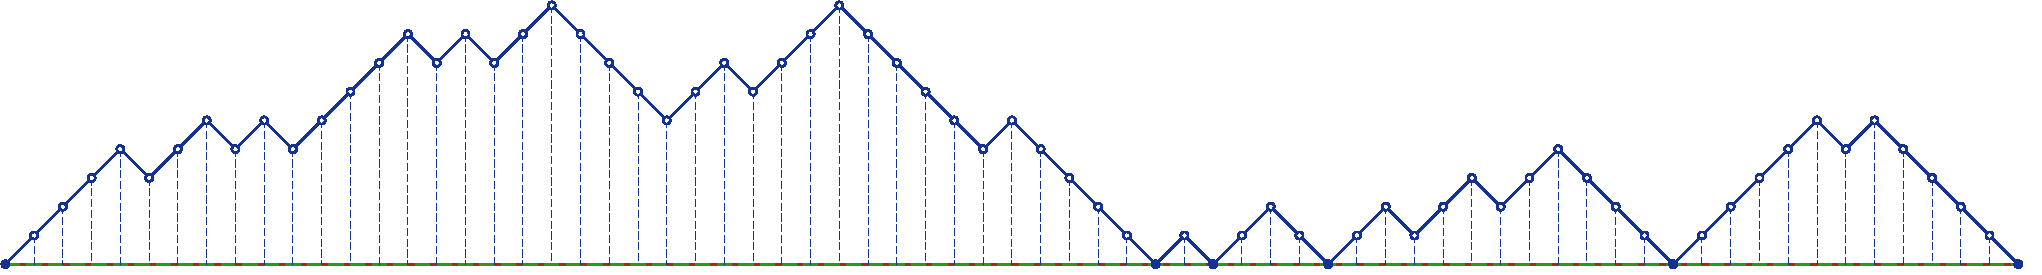
\includegraphics[width=\textwidth]{dyck/basic_dyck_path.pdf}
    \caption{Simple Dyck path with $n = 35$.}
    \label{fig:basic_dyck}
\end{figure}


\subsection{Catalan Trapezoids and Generalized Dyck Paths}
First, we define Catalan trapezoids as presented in \cite{trap}.
Let $C_k(n,m)$ be the $(n,m)^{th}$ entry of the Catalan trapezoid of order $k$,
where $C_1(n,m)$ corresponds to the Catalan triangle.

The interpretation is as follows. Consider a sequence of $n$ up-steps and $m$ down-steps,
such that the sum of any initial sub-string is not less than $1-k$.
This means that we start our Dyck path at a height of $k-1$,
and we are never allowed to cross below zero (Figure~\ref{fig:complex_dyck}).
The total number of such paths is exactly $C_k(n,m)$.
For $k = 1$, we obtain the definition of the simple Dyck path (Figure~\ref{fig:basic_dyck}).

Now, we state a result from \cite{trap} without proof
$$
C_k(n,m)=
\begin{cases}
{n+m}\choose m &0\le m<k\\
{{n+m}\choose{m}} - {{n+m}\choose{m-k}} &k\le m\le n+k-1\\
0 &m>n+k-1
\end{cases}
$$

\begin{figure}[htbp]
    \centering
    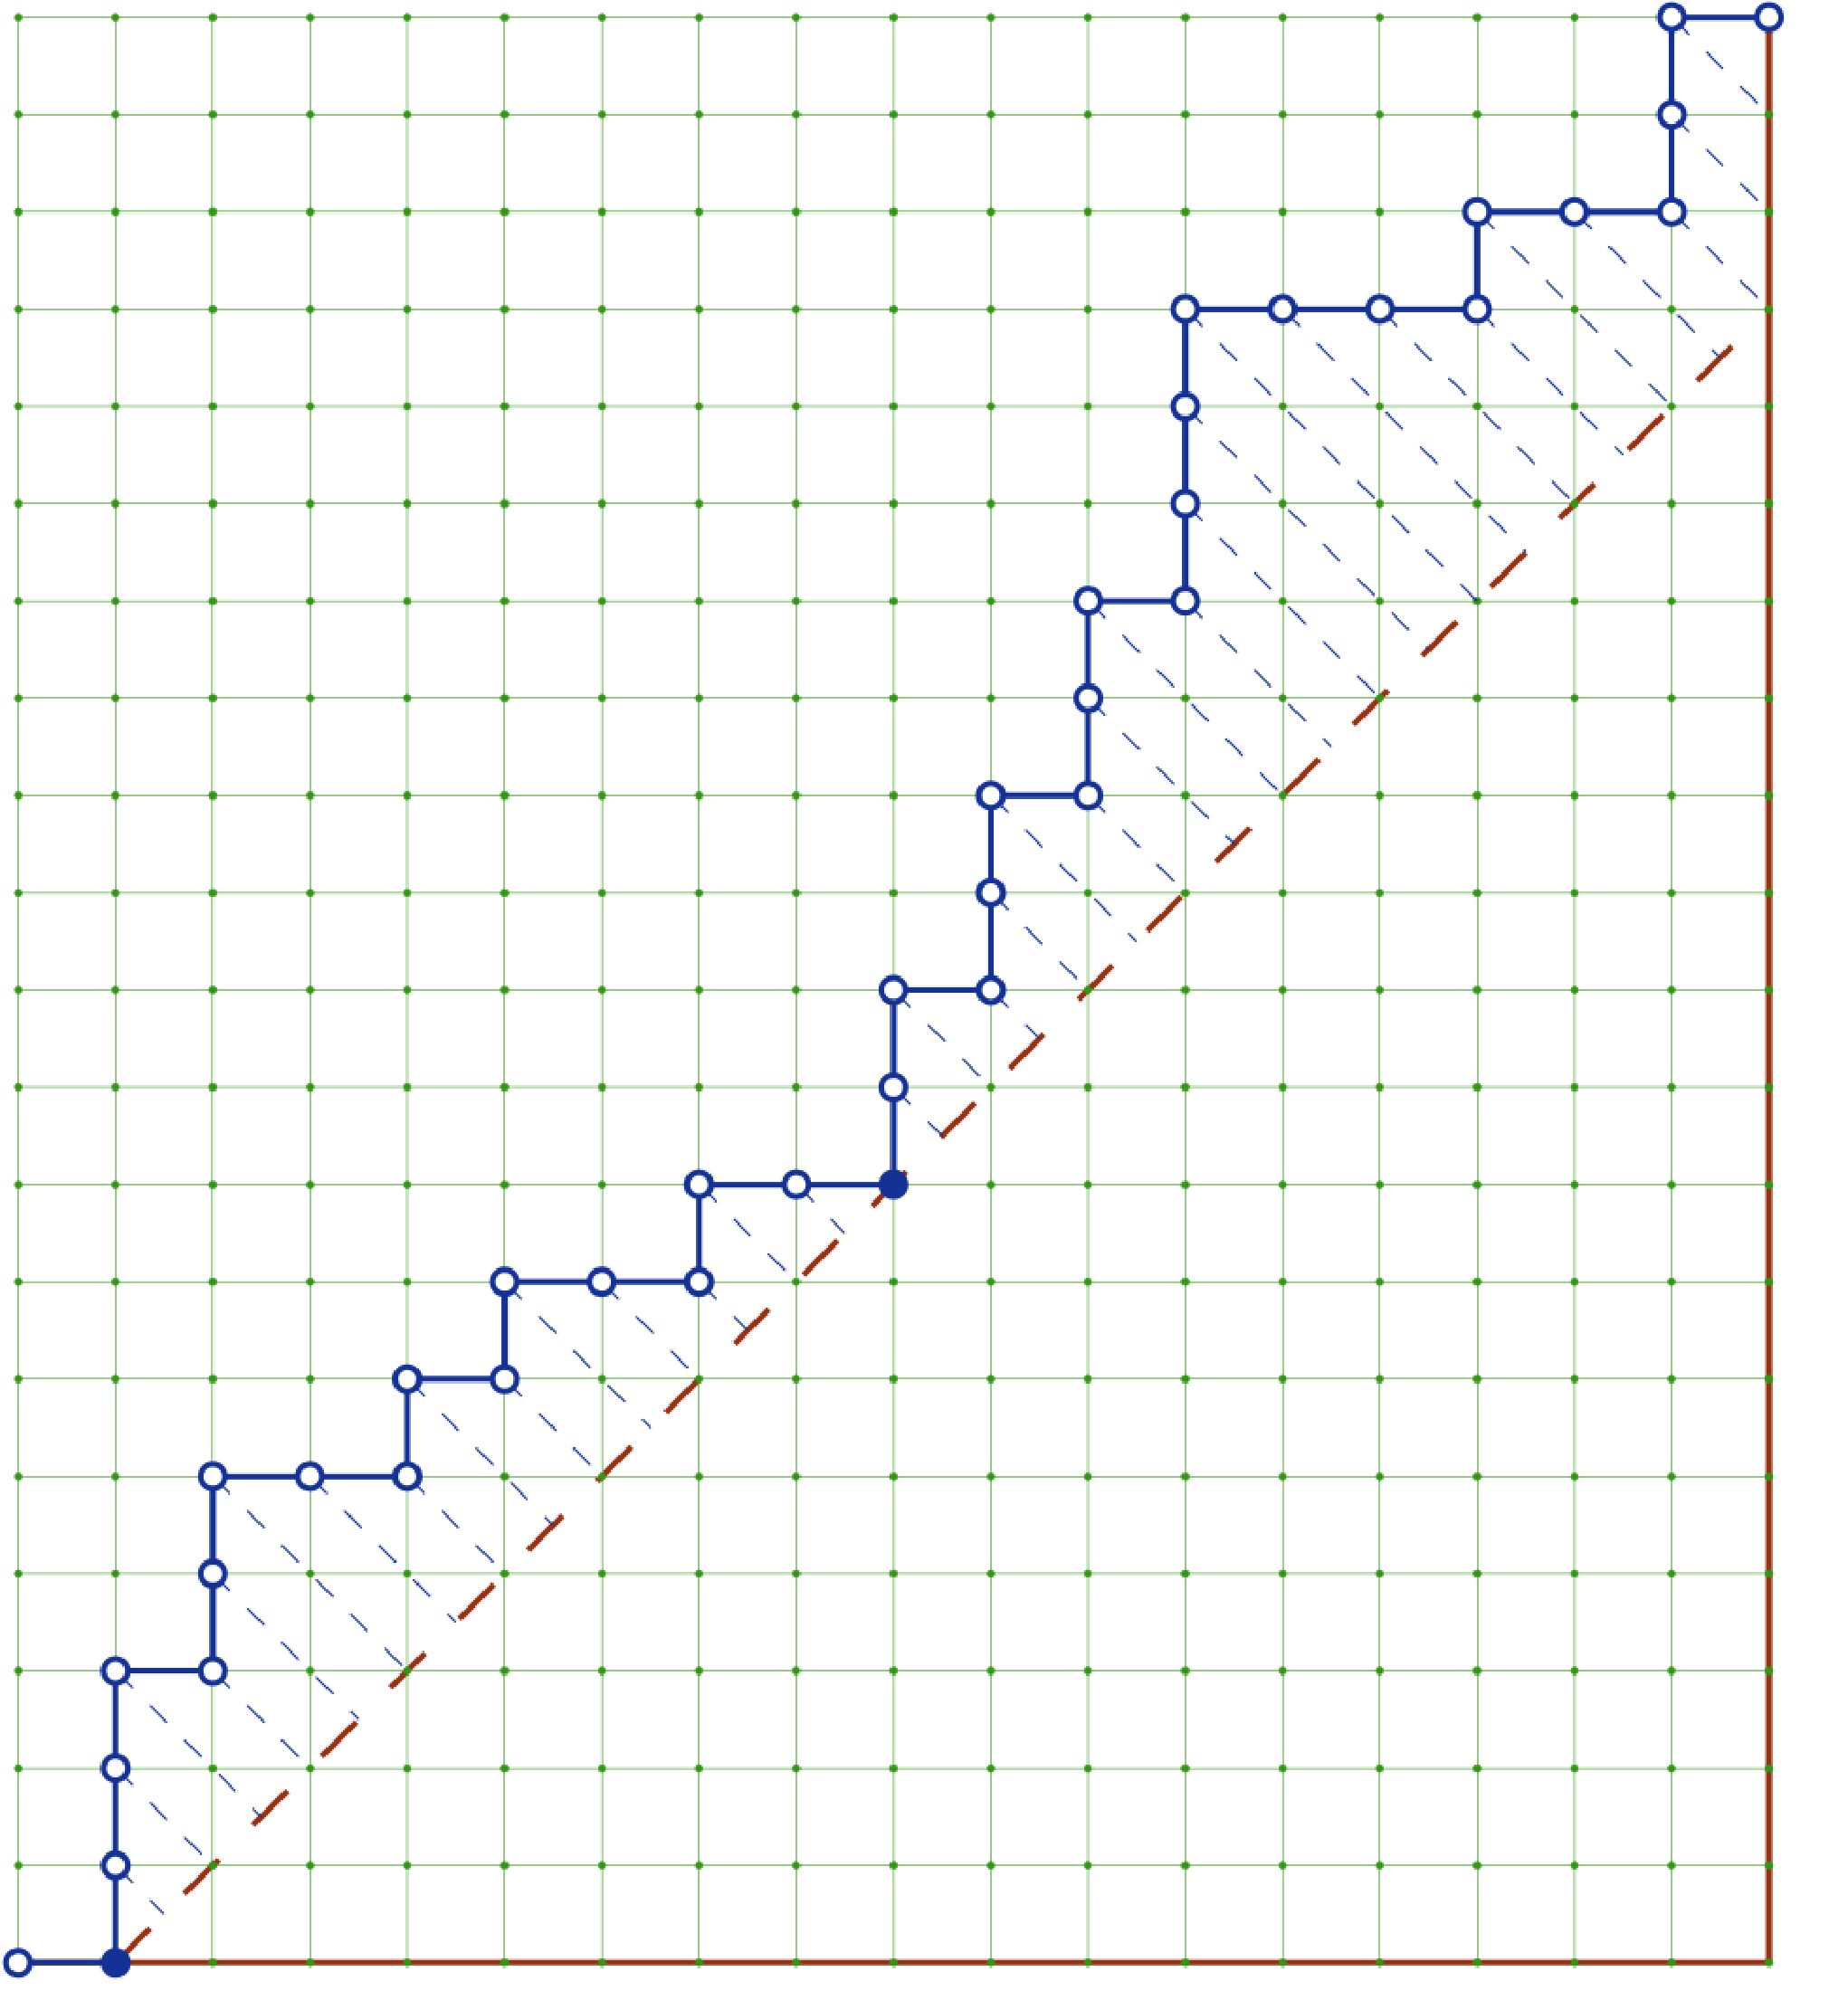
\includegraphics[width=\textwidth]{dyck/complex_dyck_path.pdf}
    \caption{Complex Dyck path with $n = 25$, $m = 22$ and $k = 3$.
             Notice that the boundary is shifted.} \label{fig:complex_dyck}
\end{figure}

\subsection{Generating Dyck Paths}
Our general recursive step is as follows.
We consider a sequence of length $2S$ comprising of $2U$ up moves ($+1$) and $2D$ down moves ($-1$).
Additionally, the sum of any initial sequence {\color{red} prefix?} canon be less than $k-1$.
Without loss of generality, let's assume that $2D\le S$. If this were not the case,
we could simply flip the sequence and negate the elements.
This essentially means that the overall Dyck path is non-decreasing.

\begin{lemma}
$S-2D = \Bo(\log n\sqrt S) \implies U-D = \Bo(\log n\sqrt S)$
\label{lem:dyck_var0}
\end{lemma}

We want to sample the height of this path after $S$ steps.
This is the same as sampling the number of $(+1)$s that get assigned to the first half of the elements in the sequence.
We define $p_d$ as the probability that exactly $D-d$ $(-1)$s get assigned to the first half.
This means that exactly $U+d$ $(+1)$s get assigned to the first half.
Consequently, the second half will contain exactly $D+d$ $(-1)$s and $U-d$ $(+1)$s.
\todo{What is $d$ is negative?}


Let us first compute this probability.
$$
p_d = \frac{D_{left}\cdot D_{right}}{D_{tot}}
$$
Here, $D_{left}$ denotes the number of valid starting sequences (first half)
and $D_{right}$ denotes the number of valid ending sequences.
Here, \textit{valid} means that each half sequence gets the appropriate number of ups and downs
and the initial sums never drop below $1-k$.
For, $D_{right}$, we will start the Dyck path from the end of the $2S$ sequence.
In this case the invalidation threshold will be a different $k'$.
This $k'$ is the final height of the $2S$ sequence. So, $k'=k+2U-2D = k+4S-2D$.
We will use this fact extensively moving forward.

Also, $D_{tot}$ is the total number of possible sequences of length $2S$, given the initial conditions.
Note that in this case the threshold remains at $k$.

We will use the following rejection sampling lemma from \cite{huge}.
\todo{Frequently?}
\begin{lemma}
\label{lem:huge}
Let $\{p_i\}$ and $\{q_i\}$ be distributions satisfying the following conditions
\begin{enumerate}
    \item There is a poly-time algorithm to approximate $p_i$ and $q_i$ up to $\pm n^{-2}$
    \item Generating an index $i$ according to $q_i$ is closely implementable.
    \item There exists a $poly(log n)$-time recognizable set $S$ such that
    \begin{itemize}
        \item $1-\SL{i\in S}{} p_i$ is negligible
        \item There exists a constant $c$ such that for every $i$, it holds that $p_i\le \log^{\mathcal{O}(1)} n\cdot q_i$
    \end{itemize}
\end{enumerate}
Then, generating an index $i$ according to the distribution $\{p_i\}$ is closely-implementable.
\end{lemma}

\begin{algorithm}[H]
    \caption{Na\"{i}ve Generator}
    \begin{algorithmic}
        \Procedure{Split}{$U, D, k$}
            \State{$S \gets U + D$}\\
            \State{$d \sim \left\{\frac{\binom{S}{S-d}\binom{S}{D+d}}{\binom{2S}{2D}}\right\}_d$}\\\\
            \State{$k' \gets k + U - D$}\\
            \State{$p_d \gets
                \frac{{{S}\choose{D-d}}-{{S}\choose{D-d-k}}{{S}\choose{U-d}}
                -{{S}\choose{U-d-k'}}}{{{2S}\choose{2D}}-{{2S}\choose{2D-k}}}$}
            \State{$q_d \gets \frac{\binom{S}{S-d}\binom{S}{D+d}}{\binom{2S}{2D}}$}\\
            \If {$p_d < q_d$}
                \State \Return $d$
            \EndIf
            \State{\textbf{draw} $X \sim\distr{Bern}(p_d/q_d)$}
            \If {$X = 0$}
                \State \Return $d$
            \EndIf
            \Return \func{Split}($U, D, k, k'$)

        \EndProcedure
        \Procedure{Height}{$x$}
            \If {$x\in heights$}
                \State \Return $heights[x]$
            \EndIf
            \State{$l \gets \func{lower-bound}(x)$}
            \State{$r \gets \func{upper-bound}(x)$}
            \State{$h_l \gets \func{Height}(l)$}
            \State{$h_r \gets \func{Height}(r)$}
            \State{$extra \gets (r-l)-(h_r-h_l)$}
            \State{$U\gets (h_r-h_l) + extra/2$}
            \State{$D\gets extra/2$}
            \State{$k\gets 1 + h_l$}
            \State{$d \gets \func{Split}(U,D,k)$}
            \State{$heights[(r+l)/2] \gets h_l + U + d$}
            \State \Return $\func{Height}(x)$
        \EndProcedure
    \end{algorithmic}
    \label{alg:naive}
\end{algorithm}

\input{dyck/height}
\subsection{Supporting ``First Return'' Queries}%
\label{sec:supporting_first_return_queries}

We might want to support more complex queries to a Dyck path.
Specifically, in addition to querying the height of a position,
we might want to know the next time the path return to that height (if at all).
We introduce a new query $\func{First-Return}(x)$ which returns the first time the walk returns to
$\func{Height}(x)$ if the step from $x$ to $x+1$ is an up-step.

The utility of this kind of query can be seen in other interpretations of Catalan objects.
For instance, if we interpret it as a well bracketed expression,
$\func{First-Return}(x)$ returns the position of the bracket matching the one started at $x$.
If we consider a uniformly random rooted tree, the fucntion effectively returns the next child of a vertex.
\todo{Explain why}

We will use the following asymptotic formula for \emph{close-to-central} binomial coefficients.
\begin{restatable}{lemma}{CentralBinomialCoefficients}
\label{lem:CentralBinomialCoefficients}
If $k = \frac{n \pm c\sqrt n}{2}$ where $c = o(n^{1/6})$,
we can approximate $\binom{n}{k}$ up to constant factors by the expression:
\[
\frac{2^n}{\sqrt n}\cdot \mathlarger e^{-c^2/2}
\]
\end{restatable}

We maintain a threshold $\mathcal T = \Theta(\log^7 n)$.
If an un-sampled interval in the Dyck path has length less than $\mathcal T$, then we sample the entire interval.
So, for intervals with length $S > \mathcal T$,
the maximum deviations are bounded by $\mathcal O(\log n\sqrt S) = \mathcal O(\log^{4.5}n)$ with high probability.
Specifically, this means that if we write the deviation as $c\sqrt n$, we see that $c = \log n$ which is $o(S^{1/6})$.
\todo{Formalize this notion of deviations}


\subsubsection{Maintaining a Boundary Invariant}%
\label{sec:maintaining_a_boundary_invariant}
\todo{Why?}
Consider all positions that have been queried already $ \langle x_1, x_2,\cdots, x_m \rangle$ (in increasing order)
along with their corresponding heights $ \langle h_1, h_2,\cdots, h_m \rangle$.
We maintain an invariant that for each $i < m$,
the Dyck path between positions $x_i$ and $x_{i+1}$ is constrained to lie above $min(h_i, h_{i+1})$.
\begin{figure}[htpb]
    \centering
    \includegraphics[width=1.0\linewidth, trim={0 12cm 0 12cm}]{images/dyck_boundary_invariant.pdf}
    \caption{Error in third segment.}
    \label{fig:dyck_boundary_invariant}
\end{figure}

It is not even clear that this is always possible.
After sampling the height of a particular position $x_i$ as $h_i$ (with $x_{i-1} < x_i < x_{i+1}$),
the invariant is potentially broken on either side of $x_i$.
We will re-establish the invariant by sampling an additional point on either side.
This proceeds as follows for the interval between $x_i$ and $x_{i+1}$
(see error in Figure~\ref{fig:dyck_boundary_invariant}):
\begin{enumerate}
    \item Sample the lowest height $h$ achieved by the walk between $x_i$ and $x_{i+1}$.
    \item Sample a position $x$ such that $x_i < x < x_{i+1}$ and $\func{Height}(x) = h$.
\end{enumerate}
Since $h$ is the minimum height along this interval, sampling the point $x$ suffices to preserve the invariant.


\subsubsection{Sampling the Lowest Achievable Height}%
\label{ssub:sampling_the_lowest_achievable_height}
For the first step, we need to sample the lowest height of the walk between $x_i$ and $x_{i+1}$.
Notice that we can assume $x_i < x_{i+1}$ without loss of generality (if $x_i > x_{i+1}$, swap them and proceed).
Let's say that the boundary is currently $k'-1$ units below $h_i$.

We know how to count the numnber of possible Dyck paths for any given boundary.
Dividing by the total number of possible paths gives us precisely the CDF we need.
This allows us to binary search to find the boundary.

We will use $D_{k}$ to denote the number of paths that respect a boundary which is $k-1$ units below $h_i$.
So, in the first step, we compute $p = D_{k'/2}/D_{k'}$.
This means that with probability $p$, the path never reaches height $h_i - k'/2$.
Otherwise, the path must reach $h_i-k'/2$ but not $h_i-k'$.
Note that we can also calculate the total number of such paths as $D_{k'} - D_{k'/2}$.
We repeat this procedure, essentially performing binary search,
until we find a $k$ such that the path reaches height $h_i-k+1$ (potentially multiple times), but never goes below it.


\subsubsection{Sampling the Position of First Return}%
\label{sec:sampling_the_location_of_first_return}
Now that we have a ``\emph{mandatory boundary}'' $k$, we just need to sample a position $x$ with height $h = x_i-k+1$.
In fact, we will do something stronger by sampling the \emph{first} time the walk touches the boundary after $x_i$.
\begin{figure}[htpb]
    \centering
    \includegraphics[width=1.0\linewidth, trim={0 6cm 0 5cm}]{images/dyck_return_sampling.pdf}
    \caption{Zooming into (and flipping) the error in Figure~\ref{fig:dyck_return_sampling}}
    \label{fig:dyck_return_sampling}
\end{figure}

We will parameterize the position $x$ the number of up-steps between $x_i$ and $x$
(See Figure~\ref{fig:dyck_return_sampling}).
This quantity will be referred to as $d$ such that $x - x_{i+1} = 2d + k-1$.
Given a specific $d$, we want to compute the number of valid paths that result in
$d$ up-steps before the first approach to the boundary.
We will calculate this quantity by counting the total number of paths to the left and right
of the first approach and multiplying them together.

Since we only care about getting a asymptotic (up to $\poly(\log n)$ factors) estimate of the probabilities,
it suffices to estimate the number of paths asymptotically as well.

\begin{restatable}{lemma}{ReturnDLeftBound}
\label{lem:ReturnDLeftBound}
If $d > \log^7 n$, then $D_{left}(d)
= \Theta\left( \frac{2^{2d+k}}{\sqrt{d}}\mathlarger e^{-r_{left}(d)}\cdot \frac{k-1}{d+k-1}\right)$
where $r_{left}(d) = \frac{(k-2)^2}{2(2d+k-2)}$.
\end{restatable}
\todo{Deal with smaller values of $d$}

\begin{restatable}{lemma}{ReturnDRightBound}
\label{lem:ReturnDRightBound}
If $U+D-2d-k > \log^7 n$, then $D_{right}(d)
= \Theta\left( \frac{2^{U+D-2d-k}}{\sqrt{U+d-2d-k}}\mathlarger e^{-r_{right}(d)}\cdot \frac{U-D+k}{U-d+1}\right)$
where $r_{right}(d) = \frac{(U-D-k-1)^2}{4(U+D-2d-k+1)}$.
\end{restatable}
\todo{Deal with other values of $d$}


\subsubsection{Estimating the CDF}%
\label{ssub:estimating_the_cdf}

\begin{restatable}{lemma}{ReturnProbabilityBoundNotNormalized}
\label{lem:ReturnProbabilityBoundNotNormalized}
$D_{left}(d)\cdot D_{right}(d)
= \Theta\left( \frac{2^{U+D}}{\sqrt{d(U+D-2d-k)}}\mathlarger e^{-r(d)}\cdot\frac{k-1}{d+k-1}\cdot\frac{U-D+k}{U-d+1}\right)$
where $r(d)=\mathcal O(\log^2 n)$.
\end{restatable}
\begin{proof}
This follows from the fact that both $r_{left}(d)$ and $r_{right}(d)$ are $\mathcal O(\log^2 n)$.
\end{proof}

\begin{corollary}
\label{cor:ReturnProbabilityRounding}
The probability $p_d$ of sampling $d$ as the number of up-steps
before the first approach to the boundary can be approximated as:
\[
p_d = \Theta\left( \frac{ 2^{U+D}\cdot\frac{(k-1)(U-D+k)}{\sqrt{d(U+D-2d-k)}(d+k-1)(U-d+1)}\cdot
\mathlarger e^{-\floor{r(d)}} }{\binom{U+D}{U}-\binom{U+D}{D-k}} \right)
\]
\todo{$D_{total}$ is not correct}
This is because the floor function only affects the value of the exponential by a factor of at most $e$.
\end{corollary}
\begin{corollary}
\label{cor:ReturnProbabilityPiecewiseContinuous}
We define a piecewise continuous function
\[
\hat q(d) = \frac{ 2^{U+D}\cdot\frac{(k-1)(U-D+k)}{\sqrt{d(U+D-2d-k)}(d+k-1)(U-d+1)}\cdot
\mathlarger e^{-\floor{r(d)}} }{\binom{U+D}{U}-\binom{U+D}{D-k}}
\]
We claim that $p_d = \Theta\left( \int\limits_d^{d+1} \hat q(d)\right)$.
Note that this integral has a closed form for a fixed value of $\floor{r(d)}$.
\end{corollary}


Let the maximum value of $r(d)$ be $r_{max} = \mathcal O(\log^2 n)$.
\begin{corollary}
\label{cor:}
We can compute the approximate normalized probabilities
\[
q_d = \frac{\int\limits_d^{d+1} \hat q(d)}{\int\limits_1^{n} \hat q(d)}
\]
such that $p_d = \Theta(q_d)$.
Furthermore, we can also compute the CDF of $q_d$ as:
\[
Q_d = \frac{\int\limits_1^{d+1} \hat q(d)}{\int\limits_1^{n} \hat q(d)}
\]
This allows us to sample from the distribution $q_d$ and use Lemma~\ref{lem:huge} to indirectly sample from $p_d$.
\end{corollary}




%\subsection{Path Segments Close to Zero}
The problem arises when we $k <\mathcal{O}(\log n)\sqrt{S}$. In this case we need to compute the actual probability,
Using the formula from \cite{trap}, we find that.
{\scriptsize
    \begin{align}
        D_{left} = {{S}\choose{D-d}}-{{S}\choose{D-d-k}}
        &&D_{right} = {{S}\choose{U-d}}-{{S}\choose{U-d-k'}}
        &&D_{tot} = {{2S}\choose{2D}}-{{2S}\choose{2D-k}}
    \end{align}
}
Here, $k' = k+2U-2D$, and so $k' = \Bo(\log n)\sqrt S$ (using Lemma~\ref{lem:dyck_var0}).

The final distribution we wish to sample from is given by $\{p_d\}_d$ where $p_d = \frac{D_{left}\cdot D_{right}}{D_{tot}}$.
To acieve this, we will use the following Lemma from \cite{huge}.
\begin{lemma}
\label{lem:huge}
Let $\{p_i\}$ and $\{q_i\}$ be distributions satisfying the following conditions
\begin{enumerate}
    \item There is a poly-time algorithm to approximate $p_i$ and $q_i$ up to $\pm n^{-2}$
    \item Generating an index $i$ according to $q_i$ is closely implementable.
    \item There exists a $poly(log n)$-time recognizable set $S$ such that
    \begin{itemize}
        \item $1-\SL{i\in S}{} p_i$ is negligible
        \item There exists a constant $c$ such that for every $i$, it holds that $p_i\le \log^{\mathcal{O}(1)} n\cdot q_i$
    \end{itemize}
\end{enumerate}
Then, generating an index $i$ according to the distribution $\{p_i\}$ is closely-implementable.
\end{lemma}

In this process, we will first disregard all values of $d$ where $|d|>\Theta(\log n\sqrt S)$.
The probability mass associated with these values can be shown to be negligible \todo{bound variance of path}.

Next, we will construct an appropriate $\{q_i\}$ and show that $p_d < \log^{\mathcal{O}(1)} n\cdot q_d$
for all $|d|<\Theta(\sqrt S)$ and some constant $c$.
We will use the following distribution
$$
q_d = \frac{{S\choose D-d}\cdot{S\choose D+d}}{{2S\choose 2D}} = \frac{{S\choose D-d}\cdot{S\choose U-d}}{{2S\choose 2D}}
$$
It is shown in \cite{huge} that this distribution is closely implementable.

First, we consider the case where $k\cdot k'\le 2U+1$.
In this case, we use loose bounds for $D_{left} < \binom{S}{D-d}$ and $D_{right} < \binom{S}{U-d}$.
We also use the following lemma (proven in Section~\ref{sec:dyck_appendix}).

\begin{restatable}{lemma}{D_tot_far_boundary}
\label{lem:D_tot_far_boundary}
When $kk' > 2U + 1$, $D_{tot} > \frac 12\cdot \binom{2S}{2D}$.
\end{restatable}

Combining the three bounds we obtain $p_d < \frac 12 q_d$.
Intuitively, in this case the dyck boundary is far away, and therefore the number of possible paths
is only a constant factor away from the number of unconstrained paths (no boundary).

The case where the boundaries are closer (i.e. $k\cdot k' \le 2U+1$) is trickier,
since the individual counts need not be close to the corresponding binomial counts.
However, in this case we can still ensure that the sampling probability is within
poly-logarithmic factors of the binomial sampling probability.
We use the following lemmas (proven in Section~\ref{sec:dyck_appendix}).

\begin{restatable}{lemma}{D_left_bound}
\label{lem:D_left_bound}
$D_{left} \le c_1 \frac{ k\cdot\log n}{\sqrt{S}}\cdot{{S}\choose{D-d}}$ for some constant $c_1$.
\end{restatable}

\begin{restatable}{lemma}{D_right_bound}
\label{lem:D_right_bound}
$D_{right} < c_2 \frac{k'\cdot log n}{\sqrt{S}}\cdot{{S}\choose{U-d}}$ for some constant $c_2$.
\end{restatable}

\begin{restatable}{lemma}{D_tot_near_boundary}
\label{lem:D_tot_near_boundary}
When $kk' \le 2U + 1$, $D_{tot} < c_3 \frac{k\cdot k'}{S}\cdot{{2S}\choose{2D}}$ for some constant $c_3$.
\end{restatable}

We can now put these lemmas together to show that $p_d/q_d \le \Theta(\log^2 n)$.
Now, we can apply Lemma~\ref{lem:huge} to sample the value of $d$,
which gives us the height of the Dyck path at the midpoint of the two given points.

\begin{theorem}
\label{thm:dyck_midpoint_sampling}
There is an algorithm that given two points at distance $a$ and $b$ (with $a < b$) along a Dyck path of length $2n$,
with the guarantee that no position between $a$ and $b$ has been sampled yet,
returns the height of the path halfway between $a$ and $b$.
Moreover, this algorithm only uses $\mathcal O(poly(\log n))$ resources.
\end{theorem}
\begin{proof}
If $b-a$ is even, we can set $S = (b-a)/2$.
Otherwise, we first sample a single step from $a$ to $a+1$, and then set $S = (b-a-1)/2$.
Since there are only two possibilities for a single step,
we can explicitly compute an approximation of the probabilities, and then sample accordingly.
Now, if $S > \Theta(\log^2 n)$ we can simply use the rejection sampling procedure described above
to obtain a $\mathcal O(poly(\log n))$ algorithm.
Otherwise, we sample each step induividually.
Since there are only $2S = \Theta(\log^2 n)$ steps, the sampling is still efficient.
\end{proof}

\begin{theorem}
\label{thm:dyck_sampling}
There is an algorithm that provides sample access to a Dyck path of length $2n$,
by answering queries of the form \func{Height}$(x)$ with the correctly sampled height of the Dyck path at position $x$
using only $\mathcal O(poly(\log n))$ resources per query.
\end{theorem}
\begin{proof}
The algorithm maintains a successor-predecessor data structure (e.g. Van Emde Boas tree)
to store all positions $x$ that have already been queried.
Each newly queried position is added to this structure.
Given a query \func{Height}$(x)$, the algorithm first finds the successor and predecessor
(say $a$ and $b$) of $x$ among the alredy queried positions.
This provides us the quarantee required to apply Theorem~\ref{thm:dyck_midpoint_sampling},
which allows us to query the height at the midpoint of $a$ and $b$.
We then binary search by updating either the successor or predecessor of $x$.
Once the interval length becomes less than $\Theta(\log^2 n)$,
we perform the full sampling (as in Theorem~\ref{thm:dyck_midpoint_sampling}) which provides us the height at position $x$.
\end{proof}



\section{Random Coloring of a Graph}%
\label{sec:random_coloring_of_a_graph}

\todo{Query access}
We wish to locally sample an uniformly random coloring of a graph.
A $q$-coloring of a graph $G = (V, E)$ is a function $\sigma : V\rightarrow [q]$,
such that for all $(u,v)\in E$, $\sigma_u \not= \sigma_v$.
We will consider only bounded degree graphs, i.e. graphs with max degree $\le \Delta$.
Otherwise, the coloring problem becomes NP-hard\todo{cite}.

Using the technique of path-coupling, Vigoda \todo{cite} showed that for $q > 2\Delta$,
one can sample an uniformly random coloring by using a MCMC algorithm.

The Markov Chain proceeds in $T$ steps. The state of the chain at time $t$ is given by $\vec X^t\in [q]^{|V|}$.
Specifically, the color of vertex $v$ at step $t$ is $\vec X^t_v$.

In each step of the Markov process, a pair $(v, c)\in V\times [q]$ is sampled uniformly at random.
Subsequently, if the recoloring of vertex $v$ with color $c$ does not result in a conflict with $v$'s neighbors,
i.e. $c\not\in \left\{ X^t_u : u\in \Gamma(v)\right\}$, then the vertex is recolored i.e. $X_v^{t+1}\leftarrow c$.

After running the MC for $T = \mathcal{O}(n\log n)$ steps we reach the stationary distribution ($\epsilon$ close),
and the coloring is an uniformly random one.

\textbf{Exact Bound:}
$t_{mix}(\epsilon) \le \left( \frac{q-\Delta}{q-2\Delta}\right)n\left( \log n + \log(1/\epsilon)\right)$
\todo{cite book (Peres, Lyons)}



\subsection{Modified Glauber Dynamics}%
\label{sub:modified_glauber_dynamics}

Now we define a modified Markov Chain that proceeds in epochs.
We denote the initial coloring of the graph by $\vec X^0$ and the state of the coloring after the $k^{th}$ epoch by $\vec X^k$.
In the $k^{th}$ epoch $\mathcal E_k$:
\begin{itemize}
    \item Sample $n = |V|$ colors $ \langle c_1, c_2,\cdots, c_n \rangle$ from $[q]$, where $c_v$ is the proposed color for vertex $v$.
    \item For each vertex $v$, we set $\vec X^k_v$ to $c_v$ if for all neighbors $w$ of $v$, $\vec X^k_w\not=c_v$ and $\vec X^{k-1}_w\not=c_v$.
\end{itemize}
%\begin{itemize}
    %\item Pick a random permutation $\pi^{(i)}$ of the vertices $V$.
    %\item Sample $n = |V|$ colors $ \langle c_1, c_2,\cdots, c_n \rangle$ from $[q]$.
    %\item Perform the standard update using the pairs $\left\langle (\pi^{(i)}_1, c_1), (\pi^{(i)}_2, c_2), \cdots, (\pi^{(i)}_n, c_n)\right\rangle$.
%\end{itemize}

This procedure is a special case of the \emph{Local Glauber Dynamics} presented in \cite{mohsen}.
The goal in \cite{mohsen} is to find a simultaneous update rule that causes few conflicts among neighbors (and converges to the correct distribution).
Notice that we can have adjacent nodes update in the same epoch, and this can also be implemented locally using \todo{what?}.
However for the sake of succinctness and because this would only improve a constant factor in the exponent,
we use their update rule and avoid a tedious path coupling argument.
\todo{Wording: a vertex needs to avoid $\le 2\Delta$ colors in order to be  accepted}

\todo{Cite Path Coupling}
For the path coupling argument, we define the standard pre-metric on the space for all possible colorings (not necessarily valid ones).
Given two colorings $X$ and $Y$, we define $d(X,Y)$ as the number of vertices $v$ such that $X_v\not= Y_v$.

We define a coupling $(X,Y)\rightarrow(X',Y')$ where $X$ and $Y$ differ only at a single vertex $v$ such that $X_v = c_X$ and $Y_v = c_Y$.
Now, we pick a random permutation of the vertices along with uniformly sampled colors:
\[
\left\langle (v_1, c_1), (v_2, c_2), \cdots, (v_n, c_n)\right\rangle
= \left\langle (\pi_1, c_1), (\pi_2, c_2), \cdots, (\pi_n, c_n)\right\rangle
\]
Now, for each $(v_i, c_i)$ in order, we update the coloring of $X$ and $Y$ as follows:
\begin{itemize}
    \item If the current color of $v_i$ as well as $c_i$ is in $\{c_X,c_Y\}$,
    then the $X$ chain picks the color $c_i$ and the $Y$ chain picks the other color.
\end{itemize}

\begin{lemma}
\label{lem:mohsen_single_epoch_distance}
If $q = 2\alpha\Delta$ and $d(X, Y) = 1$, then $\mathbb E[d(X',Y')] \le 1-\left( 1-\frac1{2\alpha}\right)e^{-3/\alpha} + \frac{1/2\alpha}{1-1/\alpha}$
\end{lemma}
\begin{corollary}
\label{cor:single_epoch_distansce}
If $q \ge 9\Delta$ and $d(X, Y) = 1$, then $\mathbb E[d(X',Y')] < \frac1{e^{1/3}}$
\end{corollary}

\begin{theorem}
\label{thm:modified_mixing_time}
If $q\ge 9\Delta$, then the Markov Chain is mixed after $\tau_{mix}(\epsilon) = 3\ln n + 3\ln(1/\epsilon)$ epochs.
\end{theorem}
\begin{proof}
\todo{Write proof}
\end{proof}




\subsection{Local Coloring Algorithm}%
\label{sub:local_coloring_algortihm}
Given a vertex $v$, the local-access generator has to output the color of $v$ after running $t \le 2\ln n$ epochs of \emph{Modified Glauber Dynamics}.
We will define the number of colors as $q = \alpha\Delta$ where $\alpha > 1$.

%Each epoch can be implemented a local generator for a permutation of $V$.
%Specifically, each epoch is a sequence of vertex and color samples:
%\[
%\chi^{(i)}
%= \left\langle (v^{(i)}_1, c^{(i)}_1), (v^{(i)}_2, c^{(i)}_2), (v^{(i)}_3, c^{(i)}_3), \cdots, (v^{(i)}_T, c^{(i)}_T)\right\rangle
%\thicksim_{\mathcal U} \left( V\times [q]\right)^T
%\]
%Here, $\left\{ v^{(i)}_1, v^{(i)}_2,\cdots, v^{(i)}_n\right\}$ is a permutation of all the vertices.
%A position $j$ in the sequence is labeled \emph{``ACCEPT''} if at the $j^{th}$ step,
%$v^{(i)}_j$ was recolored to $c^{(i)}_j$ (no conflicts with neighbors).
%Otherwise, position $j$ is marked \emph{``REJECT''}.
%We define $X^{(i)}_v = 1$ if the sample for $v$ in the $i^{th}$ epoch $(v, c^{(i)}_j)$ is accepted and $X^{(i)}_v = 0$ otherwise.

%We also define $\mathcal C^{(i)}_v$ to be the color sampled for vertex $v$ in the $i^{th}$ epoch,
%and $\mathcal I^{(i)}_v$ to be the corresponding index $j$.

Each epoch is a vector of color samples $\vec C^{i} \thicksim_{\mathcal U} [q]^n$.
Note that these values are fully independent and as such any $\vec C^i_v$ can be sampled trivially.
We also use $\vec X^i$ to denote the final vector of vertex colors at the end of the $i^{th}$ epoch.
Finally, we define indicator variables $\bm \chi^i_v$ to denote if the color for vertex $v$ was accepted at the $i^{th}$ epoch;
$\bm \chi^i_v = 1$ if and only if for all neighbors $w\in \Gamma(v)$,
we satisfy the condition $\vec  C^i_v\not= \vec X^{i-1}_w$ and $\vec C^i_v\not= \vec C^i_w$.
So, the color of a vertex $v$ after the $t^{th}$ epoch $\vec X^t_v$ is set to be $\vec C^i_v$
where $i\le t$ is the largest index such that $\bm \chi^i_v=1$.
Algorithm~\ref{alg:coloring} shows the procedure for querying the value of $\vec X^t_v$.

\begin{algorithm}[H]
\caption{Generator}
\begin{algorithmic}[1]

\Procedure{Color}{$v, t$}
    \For{$i \gets [ t, t-1, t-2 \cdots 1 ]$}
        \If {\func{Accepted}($i, v$)}
            \State \Return $C^i_v$
        \EndIf
    \EndFor
\EndProcedure

\Procedure{Accepted}{$v, t$}
    \State {$c\gets C^t_v$}
    \For{$w \gets \Gamma(v)$}
        \State {$flag\gets \ZERO$}
        \For{$t' \gets [t, t-1, t-2, \cdots, 1]$}
            \If {$t' \not= t$ \textbf{or} $\mathcal I^{(t)}_w < \mathcal I^{(t)}_v$}
                \If {$\mathcal C^{(t')}_w = c$ \textbf{and} \func{Accepted}($w, t'$)}
                    \State $flag\gets \ONE$
                    \While{$t' < t$}
                        \State $t'\gets t' + 1$
                        \If {\func{Accepted}($w, t'$)}
                            \State $flag\gets \ZERO$
                            \State \textbf{break}
                        \EndIf
                    \EndWhile
                    \If {$flag = \ONE$}
                        \State \Return $\ZERO$
                    \EndIf
                    \State \textbf{break}
               \EndIf
           \EndIf
        \EndFor
    \EndFor
    \State \Return $\ONE$
\EndProcedure

\end{algorithmic}
\label{alg:coloring}
\end{algorithm}

When the algorithm is asked for the final color of $v$, it finds the last epoch in which $v$ was accepted.
Since there are only $\mathcal O(\log n)$ epochs, we focus our attention on the subroutine $\func{Accepted}$ that samples the value of $\bm\chi^t_v$.
The algorithm iterates through the neighbors $w$ of $v$, and check for conflicts with the proposed color $c=\vec C^t_v$.
The condition $c\not= \vec C^t_w$ is can easily be checked by sampling $\vec C^t_w$ in the current epoch.
If no conflict is seen, the next step is to check whether $c\not= \vec X^{t-1}_w$.

We first iterate through all the epochs in reverse order to check whether the color $c$ was ever proposed for vertex $w$.
If not, we can ignore $w$, and otherwise let's say that the last proposal for $c$ was at epoch $t'$ i.e. $\vec C^{t'}_w = c$.
Now, we need to recursively check if this proposal was $\func{Accepted}$.
If it was, we move to epoch $t'+1$ to see if $w$'s color was replaced.
If not, we check epoch $t'+2$ and so on until we reach epoch $t-1$.
At this point we have seen that $\bm\chi^{t'}_w = 1$ (color $c$ was accepted) and every subsequent proposal until the current epoch was rejected
i.e. $\vec X^{t-1}_w = c$ and this leads to a conflict with $v$'s current proposal for color $c$ and hence $\bm\chi^t_v = 0$.
If at any of the iterations, we see that a different proposal was accepted, then $w$ does not cause a conflict and we can move on to the next neighbor.
If we exhaust all the neighbors and don't find any conflicts then $\bm\chi^t_v = 1$.

\begin{lemma}
\label{lem:color_reject_probability}
The probability that any given proposal is rejected $\mathbb P[\bm\chi^t_v=0]$ is at most $1/\alpha$.
Moreover, this upper bound holds even if we condition on all the values in $\vec C$ except $\vec C^t_v$.
\end{lemma}
\begin{proof}
A rejection can occur due to a conflict with at most $2\Delta$ possible values in $\{ C^t_w, X^{t-1}_w | w\in\Gamma(v)\}$.
Since there are $2\alpha\Delta$ colors, the rejection probability is at most $1/\alpha$.
\end{proof}

So, the number of probes required to check whether a color $c$ (assigned at epoch $t'$) was overwritten at some epoch before $t$ is:
\begin{align}
\label{eq:color_overwrite}
\Biggl[T_{t'+1} + \mathcal B\left(\frac{1}{\alpha}\right)\cdot T_{t'+2}
+ \mathcal B\left(\frac{1}{\alpha^2}\right)\cdot T_{t'+3} + \cdots
+ \mathcal B\left(\frac{1}{\alpha^{t-t'-2}}\right)\cdot T_{t-1} \Biggr]
\end{align}

\begin{lemma}
\label{lem:coloring_recurrence}
For $\alpha>4$, the expected time to sample a single $\bm\chi^t_v$ is $\mathbb E[T_t] = \mathcal{O}\left(t\Delta e^{2t/\alpha}\right)$.
\end{lemma}
\begin{proof}
We formulate a recurrence for the expected number of probes to $\{\bm\chi^{t'}\}_{t'\in[t]}$ used by the algorithm.
We will use $\mathcal B(p)$ to refer to the Bernoulli random variable with bias $p$.
When checking a single neighbor $w$, the algorithm iterates through all the epochs $t'$ such that $\vec C^{t'}_w = c$
(technically, only the last occurence matters, but we are looking for an upper bound).
If such a $t'$ is found (this happens with probability $1/q$ independently for each trial), there is one recursive call to $T_{t'}$.
Regardless of what happens, let's say the algorithm queries $T_{t'+1}, T_{t'+2}, \cdots, T_{t-1}$ until an $\func{Accepted}$ proposal is found.
Adding an extra $T_{t'}$ term to Equation~\ref{eq:color_overwrite} and summing up over all neighbors and epochs we get the following:
\begin{align}
T_{t} &\le \Delta \cdot \mathlarger\sum\limits_{t'=1}^{t} \mathbb P[C^{t'}_w = c]\cdot
\Biggl[ T_{t'} + T_{t'+1} + \mathcal B\left(\frac{1}{\alpha}\right)\cdot T_{t'+2}
+ \mathcal B\left(\frac{1}{\alpha^2}\right)\cdot T_{t'+3} + \cdots\\
&\hspace{23em}
\cdots + \mathcal B\left(\frac{1}{\alpha^{t-t'-2}}\right)\cdot T_{t-1} \Biggr]\\
&\le \Delta\cdot\mathcal B\left( \frac{1}{q}\right) \Biggl[
\mathlarger\sum\limits_{t'=1}^{t-1} T_{t'} +
\mathlarger\sum\limits_{t'=1}^{t-1} T_{t'}\cdot \left(1 + \mathcal B\left(\frac1\alpha\right) + \mathcal B\left(\frac1{\alpha^2}\right) + \cdots\right)
\Biggr]
\end{align}
In the second step, we just group all the terms from the same epoch together.
Using Lemma~\ref{lem:color_reject_probability} and the fact that $\mathbb P[C^{t'}_w = c]$ is independent of all other events,
we can write a recurrence for the expected number of probes.
\begin{align}
\mathbb E[T_t]\le \Delta\cdot\frac{1}{\alpha\Delta}
\left[
\mathlarger\sum\limits_{t'=1}^{t-1} T_{t'} + \mathlarger\sum\limits_{t'=1}^{t-1} T_{t'}\cdot
\left(1 + \frac1\alpha + \frac1{\alpha^2} + \cdots\right)
\right]
\end{align}
Now, we make the assumption that $\mathbb E[T_{t'}]\le e^{2t/\alpha}$ and show that this satisfies the expectation recurrence.
First, we sum the geometric series:
\[
\mathlarger\sum\limits_{t'=1}^{t-1} \mathbb E[T_{t'}] = \mathlarger\sum\limits_{t'=1}^{t-1} e^{2t'/\alpha}
< \frac{e^{2t/\alpha}-1}{e^{2/\alpha}-1} < \frac{e^{2t/\alpha}}{e^{2/\alpha}-1}
\]
The expectation recurrence to be satisfied then becomes:
\[
\mathbb E[T_t]\le e^{2t/\alpha}\cdot \frac 1{\alpha}\cdot \frac{1}{e^{2/\alpha}-1}\cdot \left[ 1+ \frac{\alpha}{\alpha-1} \right]
= e^{2t/\alpha}\cdot \frac{2\alpha-1}{\alpha(\alpha-1)(e^{2/\alpha}-1)} = e^{2t/\alpha}\cdot f(\alpha)
\]
We notice that $f(\alpha)$ is is upper bounded by $1$ in the domain $\alpha> 4$ (in fact $\lim\limits_{\alpha\to\infty}f(\alpha) = 1$).
This can easily be verified by taking the derivatives and using L'H\^{o}spital's rule.
Thus, our recurrence is satisfied.
Finally, we note that each probe potentially takes time $\mathcal O(t\Delta)$ to iterate through all the neighbors in all epochs
resulting in a total runtime of $\mathcal O(t\Delta e^{2t/\alpha})$.
\end{proof}

\begin{corollary}
\label{cor:coloring_improved_probes}
Instead of looking through all the epochs in order, we can use the coloring generator \todo{where?} to find the locations directly.
\end{corollary}

\begin{theorem}
\label{thm:coloring_generator_main}
Given adjacency list query access to a graph with $n$ nodes, maximum degree $\Delta$, and $q=2\alpha\Delta$ colors,
we can sample the color of any given node in an ($1/n$-approximate) uniformly random coloring of the graph in a consistent manner
using only $\mathcal O(n^{12/\alpha}\Delta\log n)$ time space and random bits.
This is sublinear for $\alpha>12$ and the sampled coloring is $1/n$-close to the uniform distribution in $L_1$ distance.
\end{theorem}
\begin{proof}
We use the mixing time from Theorem~\ref{thm:modified_mixing_time} $\tau_{mix}(1/n) = 6\ln n$ in conjunction with Lemma~\ref{lem:coloring_recurrence}.
So, the overall runtime becomes $\mathcal O(n^{12/\alpha}\Delta\log n)$.
\end{proof}




\bibliographystyle{alpha}

\bibliography{bib}


\end{document}
